% status: 0
% chapter: TBD

\title{RESTful API service to enable ease of portability leveraging libcloud}


\author{Harshad Patkar}
\affiliation{%
  \institution{Indiana University}
  \streetaddress{Smith Research Center}
  \city{Bloomington} 
  \state{IN} 
  \postcode{47408}
  \country{USA}}
\email{hpitkar@iu.edu}

\author{Sushant Athaley}
\affiliation{%
  \institution{Indiana University}
  \streetaddress{Smith Research Center}
  \city{Bloomington} 
  \state{IN} 
  \postcode{47408}
  \country{USA}}
\email{sathaley@iu.edu}

\author{Michael Robinson}
\affiliation{%
  \institution{Indiana University}
  \streetaddress{Smith Research Center}
  \city{Bloomington} 
  \state{IN} 
  \postcode{47408}
  \country{USA}}
\email{micbrobi@iu.edu}


% The default list of authors is too long for headers}
\renewcommand{\shortauthors}{H. Pitkar, S. Athaley, M. Robinson}


\begin{abstract}
Our research will measure how the portability of an application is
impacted by decisions made early in the software lifecycle when native
cloud provider APIs are used. We will demonstrate how efforts to
leverage scalable, reproducable solutions like boto and libcloud are
advantageous. We will derive reproducable code using Swagger and Python
to show how libraries like boto and libcloud can be used to migrate an
application from one cloud provider to another with a measurable
reduction in human error and with less time to execute. Additionally, we
will leverage Swagger to develop RESTful APIs to further improve the
gains. We will capture the results of the research, share the derived
code and conclude how the research can be applied to existing and new
development efforts intending to leverage cloud providers. 
\end{abstract}

\keywords{hid-sp18-518, hid-sp18-517, hid-sp18-402, libcloud}


\maketitle

\section{RESTful API service to enable ease of portability leveraging 
libcloud}\label{restful-api-service-to-enable-ease-of-portability-
leveraging-libcloud}


\subsection{Introduction}\label{introduction}

Cloud portability is a growing area of research due to the increased
profiliferation of cloud providers. Each provider has unique APIs and
tools to their cloud environments which can disincentivize portability
as it influences a consumer to stay with their existing solution
provider. Efforts to standardize cloud portability like TOSCA have made
progress yet participation by cloud providers is constrained due to the
competitive nature in the space. Each cloud provider is looking to
retain their userbase and there is also a desire by each provider to
become the de facto standard by being the market leader. To fill the
gap, solutions like Apache libcloud and boto have delivered an
abstraction solution to developers to design applications that are easy
to port.

Developers are already confronted with a lack of transparency on which
cloud provider is optimal for the long-term sustainability of their
application. Additionally, attempts to abstract away from cloud
providers are helpful yet their non-standardization still potentially
locks you into the solutions provided by Apache or communities like
boto. We will deliver a continuation of that abstraction concept with an
accepted standard, REST, to extend libcloud and boto. By leveraging
REST, we intend to introduce a standardized implementation that
leverages cloud portability libraries to manage the diversity of cloud
applications. A high-level abstract of our final concept is below.

\TODO{THis is Figure~\ref{F:arch}} and its not in PDF.

\begin{figure}[!ht]
  \centering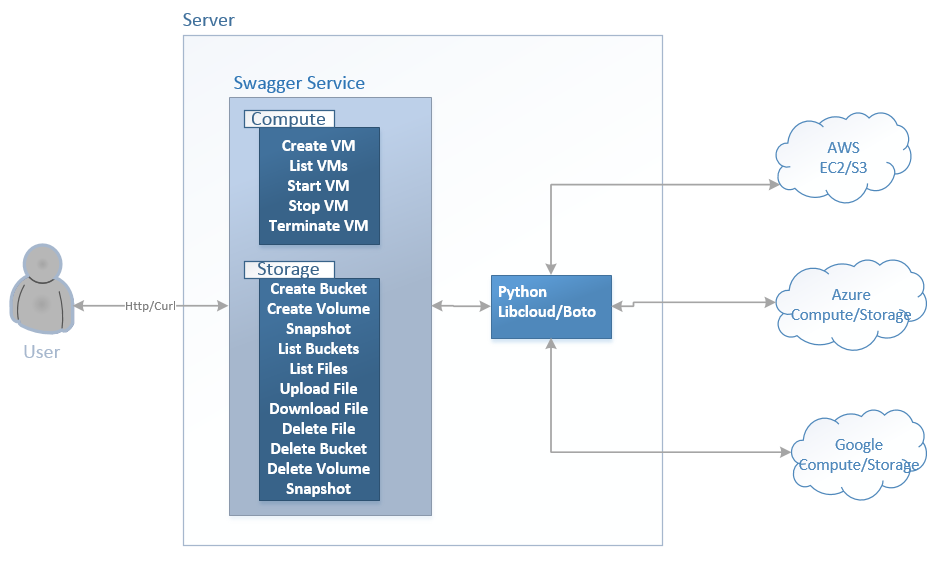
\includegraphics[width=\columnwidth]{images/proj-arch.png}
  \caption{Project Architecture}\label{F:arch}
\end{figure}


\subsection{Scope of work}\label{scope-of-work}

\begin{itemize}
\item
  Value Hypothesis
\item
  Cycle time metrics on porting a solution without boto/libcloud
\item
  Lead time metrics on use of RESTful APIs compared to command line
  usage
\item
  RESTful API

  \begin{itemize}
    \item
    Swagger development to design/build API services for UI
  \item
    Python development to leverage boto/libcloud
  \item
    Evidence of success porting a solution from/to AWS, Azure, Google
    Cloud
  \end{itemize}
\item
  Comparison of porting solution manually to libcloud/boto by command
  line
\item
  Comparison of porting solution with libcloud/boto by commandline to
  RESTful API solution
\item
  Conclusion
\end{itemize}

\hypertarget{special-consideration-to-project-format}{%
\subsection{Special Consideration to Project
Format}\label{special-consideration-to-project-format}}

\begin{itemize}
\item
  Swagger API documentation
\item
  Comparison of command line tools to Python libraries libcloud and boto
\item
  Background on TOSCA
\end{itemize}

\subsection{References}\label{references}

\begin{itemize}
\item
  D. Petcu and A. Vasilakos, \emph{Portability in Clouds: Approaches and
  Research Opportunities}, Scalable Computing: Practice and Experience,
  Vol. 15 No.~3, 2014, https://scpe.org/index.php/scpe/
\item
  Cloud Security Council, \emph{Interoperability and Portability for
  Cloud Computing}, 2017,
  http://www.cloud-council.org/deliverables/CSCC-Interoperability-and-Portability-for-Cloud-Computing-A-Guide.pdf
\item
  M. Kostoska, M. Gusev and S. Ristov, \emph{A New Cloud Services
  Portability Platform}, Procedia Engineering, Vol. 69, 2014,
  https://doi.org/10.1016/j.proeng.2014.03.118
\item
  L. Badger, D. Bernstein, R. Bohn, F. de Vaulx, M. Hogan, M. Iorga, J.
  Mao, J. Messina, K. Mills, E. Simmon, A. Sokol, J. Tong, F. Whiteside
  and D. Leaf, \emph{High-Priority Requirements to Further USG Agency
  Cloud Computing Adoption}, Special Publication 500-293,
  https://dx.doi.org/10.6028/NIST.SP.500-293
\item
  https://www.oasis-open.org/committees/tc\_home.php?wg\_abbrev=tosca
\end{itemize}


\begin{acks}

  The authors would like to thank Dr.~Gregor~von~Laszewski for his
  support and suggestions to write this paper.

\end{acks}

\TODO{There are no refernces, so latex will fail}

\bibliographystyle{ACM-Reference-Format}
\bibliography{report} 

